%\documentclass{emulateapj}
%\documentclass[preprint2]{aastex}
% \documentclass[iop]{emulateapj}
\documentclass[useAMS,usenatbib]{mn2e}
\usepackage{epsfig}
\usepackage{epstopdf}
\usepackage{lscape} % Allows landscape environment to be used
\usepackage{graphicx}
\usepackage{multirow}
\usepackage{hhline}
\usepackage{amsmath}
%\usepackage{floatrow}
%\def\gtrsim{\mathrel{\hbox{\rlap{\hbox{\lower4pt\hbox{$\sim$}}}\hbox{$>$}}}}
%\renewcommand\floatpagefraction{.9}
%\renewcommand\dblfloatpagefraction{.9} % for two column documents
%\renewcommand\topfraction{.9}
%\renewcommand\dbltopfraction{.9} % for two column documents
%\renewcommand\bottomfraction{.9}
%\renewcommand\textfraction{.1}   
%\setcounter{totalnumber}{50}
%\setcounter{topnumber}{50}
%\setcounter{bottomnumber}{50}

\begin{document}

\title[Lensing Distance]{
Scintillation Distance Measurements
}

%\author{J.~D.~Emberson\altaffilmark{1,2}, Takeshi~Kobayashi\altaffilmark{1,3} \& Marcelo~A.~Alvarez\altaffilmark{1}}
%\altaffiltext{1}{Canadian Institute for Theoretical Astrophysics,
%  University of Toronto, 60 St.George St., Toronto, ON M5S 3H8, Canada} 
%\altaffiltext{2}{Department of Astronomy and Astrophysics, University
%  of Toronto, 50 St. George, Toronto, ON M5S 3H4, Canada} 
%\altaffiltext{3}{Perimeter Institute for Theoretical Physics, 31 Caroline Street North, Waterloo, ON N2L 2Y5, Canada}
%\email{emberson@astro.utoronto.ca}

%\author{Siqi Liu\altaffilmark{1,3}, Ue-Li~Pen\altaffilmark{1,2}, J-P~Macquart\altaffilmark{4}, Walter Brisken\altaffilmark{5}, Adam Deller\altaffilmark{6}}
%\altaffiltext{1}{Canadian Institute for Theoretical Astrophysics, University of Toronto, M5S 3H8 Ontario, Canada} 
%\altaffiltext{2} {Canadian Institute for Advanced Research, Program in Cosmology and Gravitation; pen@cita.utoronto.ca}
%\altaffiltext{3} {Department of Astronomy and Astrophysics, University of Toronto, M5S 3H4, Ontario, Canada; sqliu@cita.utoronto.ca}
%\altaffiltext{4} {ICRAR-Curtin University of Technology, Department of Imaging and Applied Physics, GPO Box U1978, Perth, Western Australia 6102, USA; J.Macquart@curtin.edu.au}
%\altaffiltext{5} {National Radio Astronomy Observatory, P.O. Box O, Socorro, NM 87801, USA; wbrisken@aoc.nrao.edu}
%\altaffiltext{6} {ASTRON, the Netherlands Institute for Radio Astronomy, Postbus 2, 7990 AA, Dwingeloo, The Netherlands; deller@astron.nl}
\author[Liu et al]{Siqi Liu$^{1,3}$\thanks{E-mail:\ sqliu@cita.utoronto.ca}, Ue-Li
  Pen$^{1,2}$\thanks{E-mail:\ pen@cita.utoronto.ca}, J-P Macquart$^{4}$\thanks{E-mail:J.Macquart@curtin.edu.au},
  Walter Brisken$^{5}$\thanks{Email:wbrisken@aoc.nrao.edu}, Adam Deller$^{6}$\thanks{E-mail:deller@astron.nl}\\
 $^1$ Canadian Institute for Theoretical Astrophysics, University of Toronto, M5S 3H8 Ontario, Canada \\
$^2$ Canadian Institute for Advanced Research, Program in Cosmology
and Gravitation\\
$^3$ Department of Astronomy and Astrophysics, University of Toronto, M5S 3H4, Ontario, Canada\\
$^4$ ICRAR-Curtin University of Technology, Department of Imaging and Applied Physics, GPO Box U1978, Perth, Western Australia 6102, USA \\
$^5$ National Radio Astronomy Observatory, P.O. Box O, Socorro, NM 87801, USA\\
$^6$ ASTRON, the Netherlands Institute for Radio Astronomy, Postbus 2, 7990 AA, Dwingeloo, The Netherlands\\
}

\date{\today}

\pagerange{\pageref{firstpage}--\pageref{lastpage}} 
\pubyear{2015}

\maketitle
\label{firstpage}
\begin{abstract}
We show how interstellar scintillations, combined with VLBI
measurements, can be used to measure distances.  
We apply the technique to archival data on PSR
B0834+06, concluding that for this example the plasma lenses can be
precisely modelled using the Pen and Levin (2014) inclined sheet model,
resulting in two distinct lens planes.  This data strongly favours the
reconnection sheet model over turbulence as the primary source of
pulsar scattering. A global 
conformal distance degeneracy exists which allows a rescaling of the
absolute distance scale.  This degeneracy is broken if the pulsar resides in a
binary system, which is the case for most precision timing targets.
\end{abstract}
\begin{keywords}
Pulsar
\end{keywords}

\newcommand{\be}{\begin{eqnarray}}
\newcommand{\ee}{\end{eqnarray}}
\newcommand{\beq}{\begin{equation}}
\newcommand{\eeq}{\end{equation}}

\section{Introduction}

Pulsars have long provided a rich source of astrophysical information
due to their compact emission and predictable timing. One of the
weakest measurements for most pulsars is their direct geometric
distance.  For some pulsars, timing parallax or VLBI parallax has
resulted in direct distance determinations.  For most pulsars, the
distance is a major uncertainty for precision timing interpretations,
including mass, moment of inertia, and gravitational wave
direction \citep{boyle2012}.

Direct VLBI observation of PSR B0834+06 shows multiple images lensed
by the interstellar plasma.  Combining the angular positions and
scintillation delays, the authors published the derived effective
distance \citep{2010ApJ...708..232B} of approximately $1168\pm 23$ pc
for apexes whose time delays range from $0.1$ ms to $0.4$ ms, and
$1121\pm 59$ pc for $1$ ms apexes.  This represents a precise
measurement compared to all other attempts to derive distances to this
pulsar.  This effective distance is a combination of pulsar-screen and
earth-screen distances, and does not allow a separate determination of
the individual distances.  A binary pulsar system would in principle
allow a breaking of this degeneracy \citep{2014MNRAS.442.3338P}. One
potential limitation is the precision to which the lensing model can
be understood.  In this paper, we demonstrate that the lensing screen
consists of nearly parallel linear refractive structures, in two
screens.  The precise model confirms the one dimensional nature, and
thus the small number of parameters that need to be measured to
quantify the lensing screen. 

\section{Lensing}
\subsection{B0834+06}

Our analysis is based on the reduced apex catalog from
\citet{2010ApJ...708..232B}. Other information from each identified apex includes delay,
delay rate, RA and dec, one for each of $4$ $8$ MHz wide sub-bands, centering $314.5$ MHz, $322.5$ MHz, $328.5$ MHz and $334.5$ MHz.  We mapped
a total of $9$ apexes from the $0.4$ ms group, and $5$ from the $1$ ms
group. This results in an estimation
for the mean value and standard deviation, which are listed in Table
\ref{table:apex}. The time is calculated with $2{\tau}f/{f_{D}}$,
which is equivalent to pulsar moving at $640$pc plane from the
original position to the lensed image position with the velocity
calculated. How distance of the pulsar is related to the time delay and how velocity is related to the differential frequency is defined by the following equations:

\begin{align*}
\tau &=\frac{D_{\rm e}{\theta}^2}{2c}, \\
f_D  &=f\cdot\frac{\delta\tau}{dt},
\end{align*} 
where ${D_{\rm e}}$ is the effective distance, equivalent to the lens placing at the middle point of the pulsar: $D_{\rm e}={D_p D_s}/({D_p - D_s})$. 

A least square effective distance results in
$D_e^M=1017.1\pm 2.8$ for the main 0.4\ ms apexes and
$D_e^S = 1243 \pm 64$ for the secondary 1\ ms apexes. This seems to
indicate that the secondary screen is closer to the pulsar. The error
bars are large enough to allow them to be at the same distance, or
perhaps a reverse distance ordering.  In this paper, we present two
analyses for comparison: equidistant, and at the best fit distances.
In the first case, no direct distance measurement is possible, but it
nevertheless illustrates a robust interpretation of the data.


\subsection{Lens Solution}

In order to interpret the data, we adopt the lensing model of
\citet{2014MNRAS.442.3338P}.  In the absence of a lens model, the
fringe rate, delay and angular position cannot be uniquely related. In
this model, the lensing is due to projected fold caustics of a thin
sheet closely aligned to the line of sight.

%From time delay $\tau$ and the angular position of the pulsar, we obtained the effective distance of the pulsar as follows: 
%for $0.4$ ms group, $D_{\rm e}=1017\pm2.8$\ pc; 
%and for $1$ ms group, $D_{\rm e}=1121\pm64$\ pc.
Furthermore, if we know the distance of the pulsar is $640$ pc by parallax,
the screen where $0.4$ ms scintellation points are refracted, $D_s$ is equal to $392.8$ pc. We know the position of the axis angle, with an $\alpha$ 25.2 degree west of north, and the positions of the $0.4$ ms pile are calculated. They are marked out with the scatter points on the left sidde of Figure \ref{Doublelens}.
Similarly, for $1$ ms apexes, the $D_s$ is equal to $422.5$ pc. Thus, the degeneracy of the distance of the screen is broken.

For the positions of the $1$ ms apexes. First, matching the $\theta$-$\tau$ relation, which is plotted in Figure \ref{thetatau}, we calculated the $\theta$ from observation $\tau$. Second, we consider the point with the largest $\theta$ among this $1$ ms group, which is called 5, share the same $\theta_{\parallel}$ with the point with the largest $\theta$ among the $0.4$ ms group, which is called 6. Thus, the position of point 5, is determined. Third, to determine the position of the rest point $1-4$, we need to know the velocity of the pulsar, and then to fit the RA and dec to get the same differential frequency with the observation. To know the proper motion of the pulsar, we calculated the its component in two directions: $v_{\parallel}$ according to the differential frequency of point $6$ in $0.4$ ms; and $v_{\rm A5}$ (in the direction pointing from point 5 to A) according to the differential frequency of point $5$. Fourth, we fit the position of the rest four points, with known proper motion of the pulsar. Then we fit a line to this five calculated points. 
%Lying on the fitted line, point 5 share the same $\theta_{\parallel}$ as the point with the largest $\theta_{\parallel}$ in the $0.4$ ms apexes. Solving the differential frequency ${f_D}$ of this point, we can calculate the relative velocity of this point to the pulsar, called vA2, which is in the plane that is perpendicular to our line of sight with a direction pointing from point 5 to the position of the pulsar. With the same method, we obtained the $v_{\parallel}$ from the $0.4$ ms data. Thus, the total velocity of the pulsar is determined.

That is one lens model fitting. Knowing time delay ${\tau}$ , we can get the distance of the screen; knowing the position of point 5 and the differential frequency ${f_D}$, we can get the velocity of the pulsar; knowing the velocity and observation diffferential frequency, we can get the position of points $1-4$.

\subsection{Discussion of one lens model}

The $0.4$ ms group lens solution appears consistent with the premise of the inclined
sheet lensing model \citep{2014MNRAS.442.3338P}.

For $1$ ms group, the secondary lens
only images a subset of the primary lens images.  This could happen if
the secondary lens screen is just under the critical inclination
angle, such that only $3-\sigma$ waves lead to a fold caustic.  If the
primary lens were at a critical angle, the chance of encountering a
somewhat less inclined system is of order unity.
%For the $0.4$ ms apexes, the one lens model could perfectly interpret the observation. 
More surprising is the absence of a single refraction
image of the pulsar, which is expected at position J.  This could
happen if the maximum refraction angle is just below critical, such
that only rays on the appropriately aligned double refraction can form
images.  This scenario predicts that at frequencies just below $300$
MHz, or a few weeks earlier in time, the pulsar should be seen at
position J. We made a plot of the refraction angle $\beta$ in the
direction that is transverse to the first lens plane in Figure
\ref{vtrans}.  From our calculation, it takes $22$ days for the puslar
to move from point 1 on the near screen to J, and it takes $44$ days
for the pulsar to move from point 5 on the near screen to J.  The data
spans about 10\% in frequency, making it unlikely that single lens
image J would not be seen due to the larger required refraction
angle.  Instead, we speculate that the fold caustic could have formed
near double lens image 1, and thus only intersections with the closer
lens plane caustic south of image 1 are double lensed.

\subsection{Double lens model}
The $v_{\parallel}$ to the plane should be equal. While for the calculated positions of $1$ ms apexes, they do not. The plane where the light was refracted should be transverse to the line that connects the pulsar and the lensed image. For the approximately same time delay of the $5$ points among $1$ ms group, the lens where the image formed should be at the same distance away from us. The only reasonable plane is line that fits all these five points, marked with a solid line in Figure \ref{Doublelens}.  However, in this senario, the screens cross each other, which is unrealistic for the structure of the interstellar medium. 
%Thus, on the plane which is perpendicular to our line of sight, the incoming line should be in agree with the refraction line.
% If the light of the pulsar are being refracted by one interstellar medium lens, they should be distributed along a line like the axis of the $0.4$\ ms group, and we already know that all $1$ ms lensed images lie on the solid line in Figure \ref{Doublelens}, the only possible position will be J, which is the pedal of the position of the pulsar to the screen. 

Therefore, we consider another model candidate: the double lens model. Respective calculation shows that the light is first refracted by the far screen and then refracted by the near screen. 

The first step is to calculate the position of J. We calculated the position of J by matching the time delay of point 2, point 4 and point 5. The result shows that the far lens is $425$ pc away from us. And its position is marked in Figure \ref{Doublelens}. Because J is the pedal to the far screen, we made a line that is perpendicular to AJ, the solid line in Figure \ref{Doublelens}.
%calculate the position of the far lens (lens $1$) and the near lens (lens $2$). As what has been discussed previously, the solid line is considered to be the far lens, where the positions have a larger effective distance. And the near lens is considered to be the lines that is perpendicular to the $0.4$ ms group axis. 

The second step is to find the matched pairs of those two lenses. By try and error, we found that the 5 points in $0.4$ ms group that have the largest $\theta$ should be the candidates where the near lens lie.  These five matched lines are marked with dot dash lines in Figure \ref{Doublelens} and their values are listed in Table \ref{table:double_lens_compare} the first two columns. They are the secondary screens, at a distance $392.8$ pc away from us. 
%We calculated with the distance of the screen which is calculated in the one lens model, and then move the distance of the far screen little by little to make the calculated time delay match the observation resul

By using the refraction law, we solve the solutions in double lens model.And the solved positions are plotted in Figure \ref{Doublelens}, and respective time delays and differential frequencies are listed in Table \ref{table:double_lens_compare}.  Figure \ref{first_reflect} and Figure \ref{second_reflect} are examples of how light are being refracted on the first lens plane and the second lens plane, with $\theta_{\parallel}$ equal to $-17.44$ mas of the secondary lens plane position.



%table one for 1ms positions

\begin{table*}
\centering
%\label{apex1ms}
%\resizebox{!}{1cm}{
\begin{tabular}{llllllllll}
\hline
$\theta_{\parallel}$(mas) &$f_D$(mHz) & $\sigma_{f_D}$(mHz) & $\tau$(ms) & $\sigma_{\tau}$(ms) & RA(mas) & $\sigma_{RA}$(mas) & dec(mas) & $\sigma_{dec}$(mas) & time(day)\\
\hline
 -8.29   & -12.94                            & 0.19      & 0.0845  & 0.0005          & 2.87    & 0.11                                     & -8.201     & 0.088      & 49.9                                \\

-10.71   &-16.80                             & 0.28      & 0.14123 & 0.0009         & 3.86    & 0.07                                     & -10.563    & 0.053      &64.5                                \\

-12.36   &-18.92                            & 0.23      & 0.188   & 0.002           & 5.06    & 0.20                                      & -10.58    & 0.13      &74.4                        \\

-13.44 & -20.40                             & 0.49      & 0.222   & 0.003           & 5.55    & 0.30                                      & -11.73    & 0.21      &80.8                                \\

-13.86 &-21.17                            & 0.61      & 0.236   & 0.002           & 5.12    & 0.43                                     & -12.56    & 0.31      &83.4                                \\

-14.63   &-22.32                            & 0.47      & 0.2633  & 0.0003          & 6.16    & 0.14                                     & -14.15    & 0.10       &88.0                                \\

-16.29   &-24.63                            & 0.40       & 0.327  & 0.003          & 6.49    & 0.29                                     & -14.06    & 0.20       &98.0                                \\

-16.57  &-24.94                            & 0.44      & 0.338 & 0.0003         & 8.29    & 0.42                                     & -14.37    & 0.32      &99.7                                \\

-17.44   &-26.09                            & 0.36      & 0.3743 & 0.0006         & 8.53    & 0.52                                     & -15.74    & 0.42      &105                               
\\ \hline 
 $\cdots$ &       -35.06                           & 0.52                               & 0.950               & 0.002                              & -15.23  & 0.69                                     & -21.06   & 0.70   &202                                   \\

$\cdots$     & -38.31                           & 0.64                               & 0.9763              & 0.0009                             & -15.02  & 0.48                                    & -20.74   & 0.38  &190                                    \\

  $\cdots$  &-40.17                           & 0.55                               & 1.0045              & 0.008                             & -14.14  & 0.66                                    & -22.27   & 0.62  &187                                   \\

  $\cdots$ &-41.27                           & 0.54                               & 1.037              & 0.003                              & -11.28  & 0.93                                     & -19.2   & 1.1   &188                                   \\

$\cdots$ & -43.08                           & 0.44                               & 1.066              & 0.005                              & -8.4   & 1.7                                      & -24.1   & 1.4   &185   \\
 \hline                                 
\end{tabular}
\label{table:apex}
\caption{0.4ms and 1ms observation positions.}
\end{table*}

\begin{table*}
\centering
\resizebox{\linewidth}{!}{
\begin{tabular}{llllllll}
\hline
Lens 1 $\theta_{\parallel}(mas)$ & Lens 2 $\theta_{\parallel}$(mas) & Observation $\tau$(ms) & $\sigma_\tau$(ms)  & Calculated $\tau$(ms) & Observation $f_D$(mHz)  &$\sigma_{f_D}$(mHz)      & Calculated $f_D$(mHz) \\ \hline
-13.86  & -12.71 &   0.950     &0.002    & 0.955       & -35.06     &0.52 & -37.22 \\ 
-14.63  & -14.69 &  0.9763    &0.0009   & 0.9763       & -38.31 &0.64   & -38.31 \\ 
-16.29  & -15.78 &  1.005    &0.008   & 1.0272      & -40.17 &0.55    & -40.64 \\ 
-16.57  & -16.35 &   1.037     &0.003    & 1.036        & -41.27 &0.54   & -41.04 \\ 
-17.44  & -17.44 & 1.066     &0.005    & 1.066         & -43.08 &0.44  &-42.26 \\ \hline
\end{tabular}
}
\label{table:double_lens_compare}
\caption{comparison of the observation time delay and the differential frequency of the observation data and the calculated result of double lens model.}
\end{table*}
%\end{table}


%\begin{figure*}
%\centering
%\epsscale{1.0}
%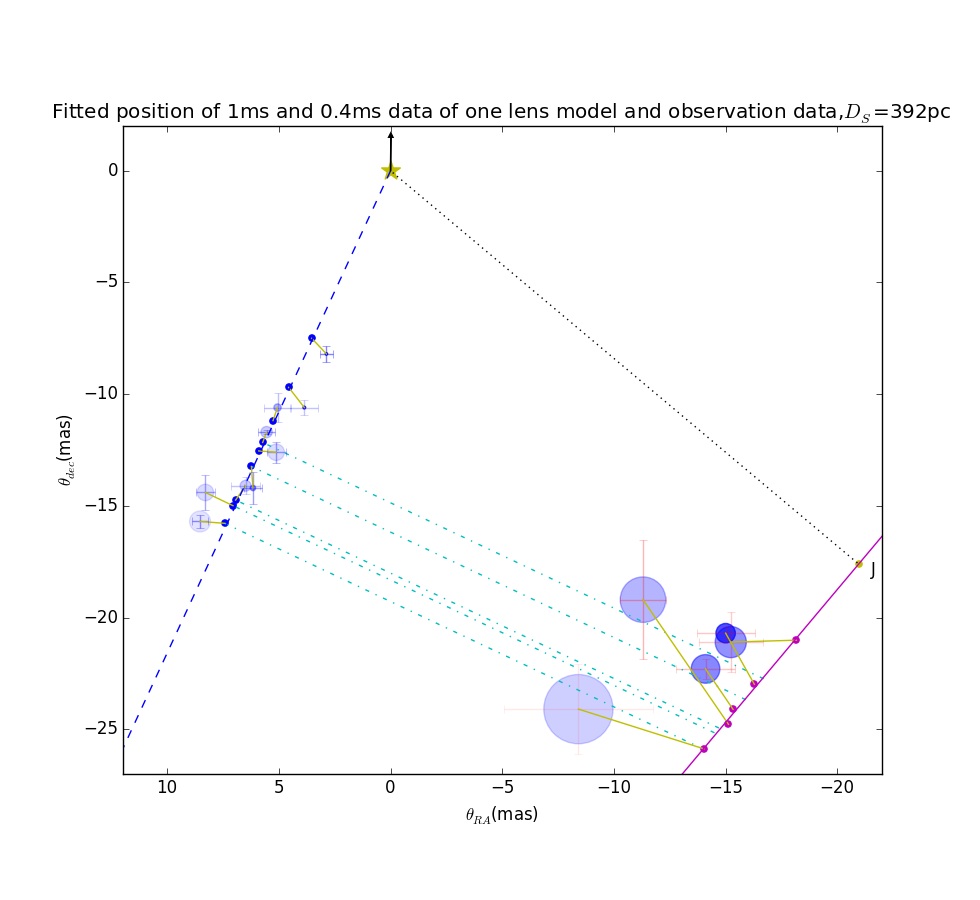
\includegraphics[width=0.8\textwidth, angle=0]{One_lens_640_392_392.png}
%\includegraphics{zN.eps}
%\caption{Fitted position of $1$ms and $0.4$ms data of one lens model and observation data. In both apexes regions, the position of the screen locate at $392.82$pc. Blue points on the left side are the points that fitted from the $f_D$ and $\tau$ of from the $0.4$ms observation. Blue line is the fitted line of $0.4$ms apex positions, with a $25.2$ degree west of the north. The points lie on the left side with errorbars, are the observation points together with their sample errors; while the transparent circles are plotted with population errors, where smaller transparent data are darker. Short solid lines between them are the matched positions of the apexes in $1ms$ region and $0.4ms$ region, which share the same $\theta_{\parallel}$. The points on the right side are the points that fitted from the $f_D$ and $\tau$ of the $1$ms observation with an avearage of four bandwidths. Solid line is the fitted line of these positions. Those points with errorbars nearby are the observation points together with their sample errors, while the transparent circles are plotted with population errors. The dotted line on the top right side is vertical to the solid line. Short solid lines connect the observation points and the fitted positions. Middle lines connect the $0.4$ms and $1$ms fitted positions with the same $\theta_{\parallel}$. The velocity of the pulsar is $199981$m/s, with a degree $0.0007$ radian east of north, which is marked out at the top of the figure.  }
%\label{Onelens_392}
%\end{figure*}

%\begin{figure*}
%\centering
%\epsscale{1.0}
%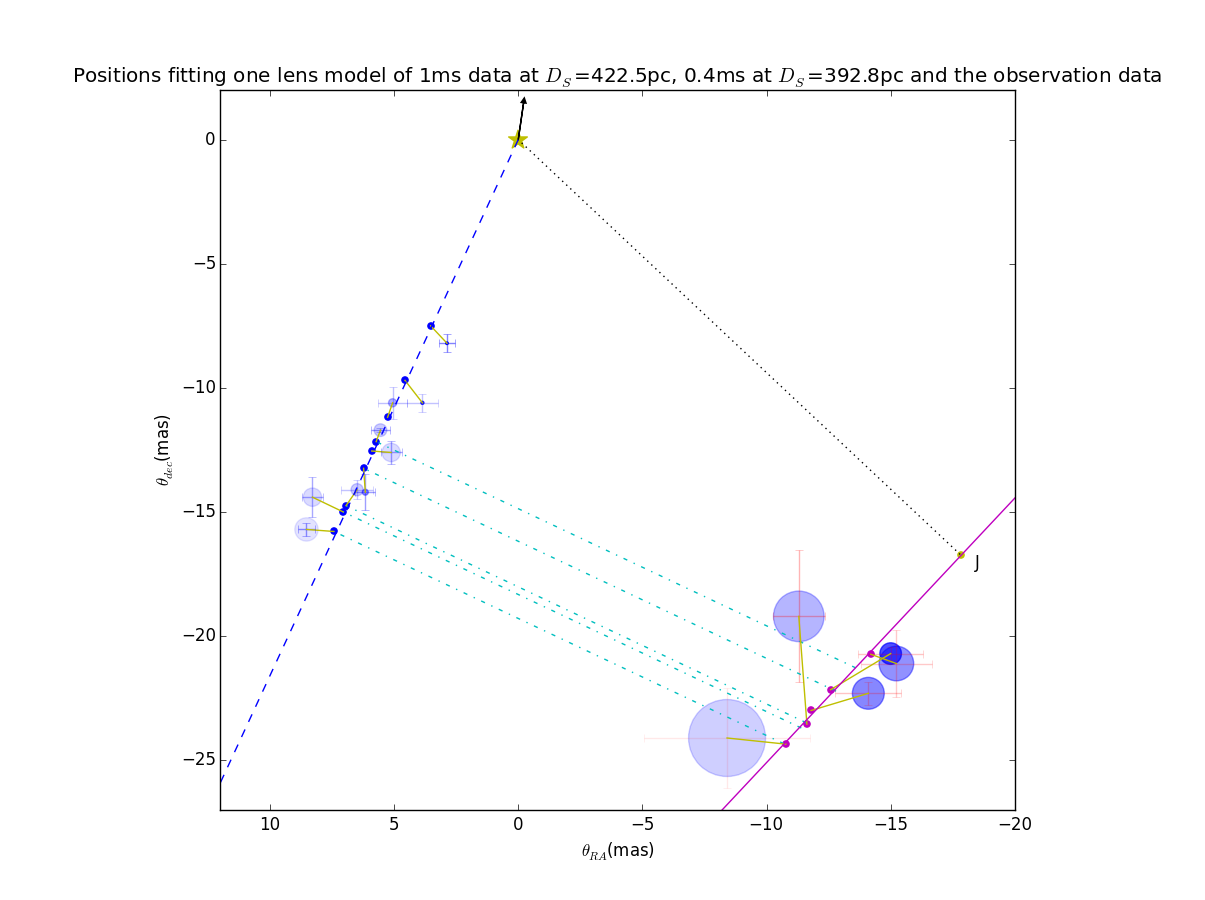
\includegraphics[width=0.8\textwidth, angle=0]{One_lens_640_392_422.png}
%\includegraphics{zN.eps}
%\caption{Same Observation data with the previous plot, this time we put the points with time delay lie in the range $1$ms at the screen that is $422.5$ pc away from us, which fitts better with the observation data. Velocity in this situation is $188499$m/s, with an angle $0.144147$ radian west of north. }
%\label{Onelens_392_422}
%\end{figure*}

\begin{figure}
\centering
%\epsscale{1.0}
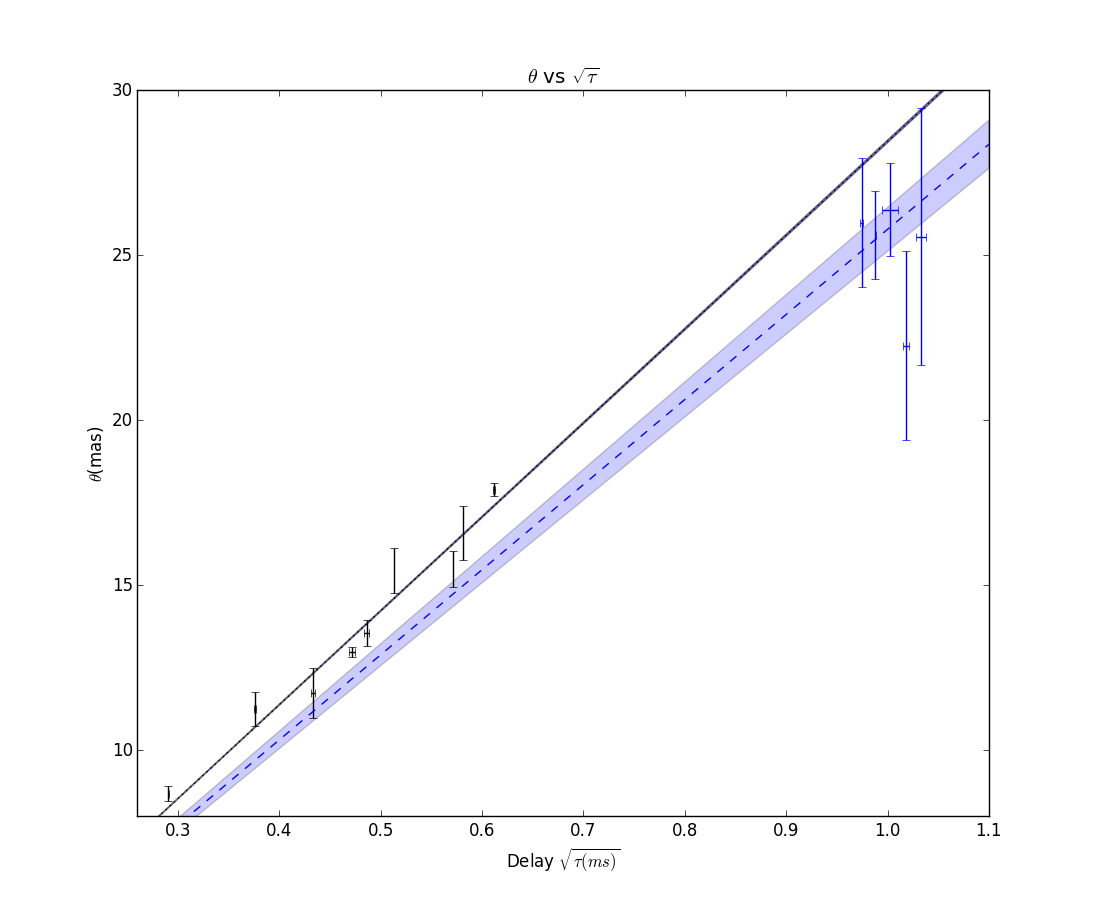
\includegraphics[width=1.0\linewidth, angle=0]{Theta_tau.png}
\caption{${\theta}$ vs ${\sqrt{\tau}}$. The solid line is the fitted line of the 0.4ms positions, where $k=28.51$ with an error region of $\sigma_k=0.04$. The dashed lines are the fitted lines of the 1ms position, where $k=25.78$ with an error region of $\sigma_k=0.66$.
}
\label{thetatau}
\end{figure}








%\begin{figure*}
%\centering
%\epsscale{1.0}
%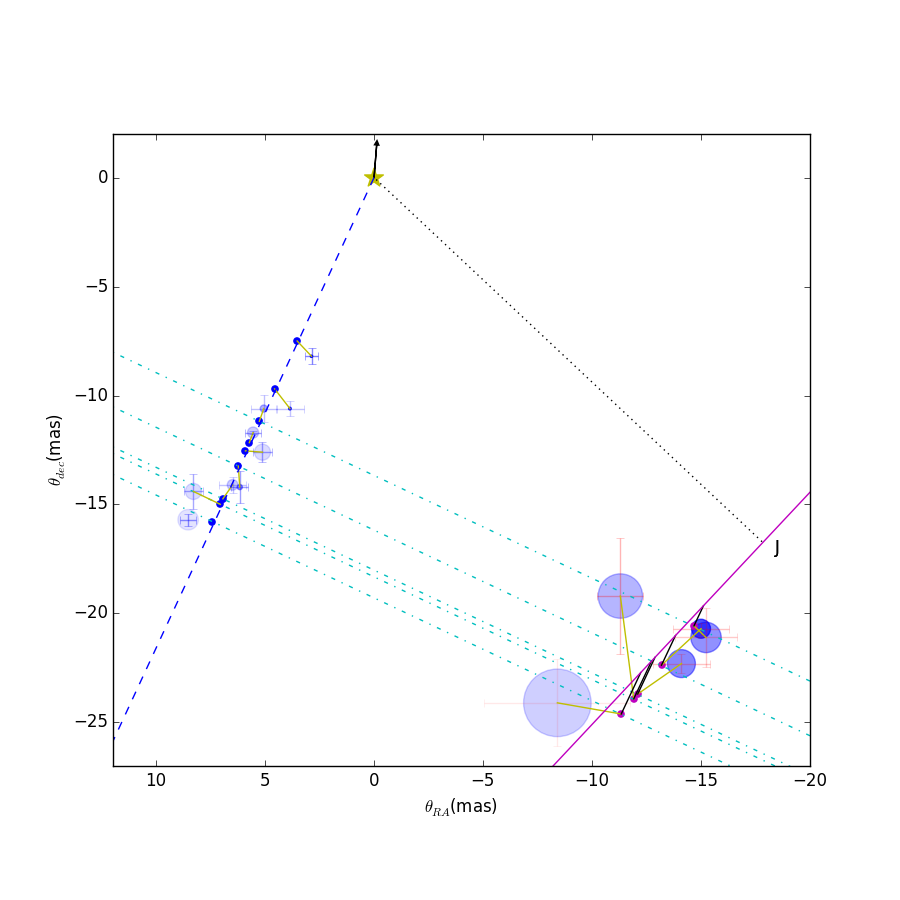
\includegraphics[width=1.0\textwidth, angle=0]{Double_lens_640_425_392.png}
%\caption{Fitted position of $1$ms and $0.4$ms data of double lens model and observation data.In both apexes regions, the position of the screen locate at $392.82$pc and $425$pc. Blue points on the left side are the points that fitted from the $f_D$ and $\tau$ of from the $0.4$ms observation. Blue line is the fitted line of $0.4$ms apex positions, with a $25.2$ degree west of the north. The points lie on the left side with errorbars, are the observation points together with their sample errors; while the transparent circles are plotted with population errors, where smaller transparent data are darker. Short solid lines between them are the matched positions of the apexes in $1ms$ region and $0.4ms$ region, which share the same $\theta_{\parallel}$. The points on the right side are the points that fitted from the $f_D$ and $\tau$ of the $1$ms observation with an avearage of four bandwidths. Solid line is the fitted line of these positions. Those points with errorbars nearby are the observation points together with their sample errors, while the transparent circles are plotted with population errors. The dotted line on the top right side is vertical to the solid line. Short solid lines connect the observation points and the fitted positions. Middle lines connect the $0.4$ms and $1$ms fitted positions with the same $\theta_{\parallel}$. The velocity of the pulsar is $191.4$km/s, with a degree $5.56$ degree west of north, is also marked out at the top of the figure.  }
%\label{Doublelens}
%\end{figure*}

\begin{figure*}
\centering
%\epsscale{1.0}
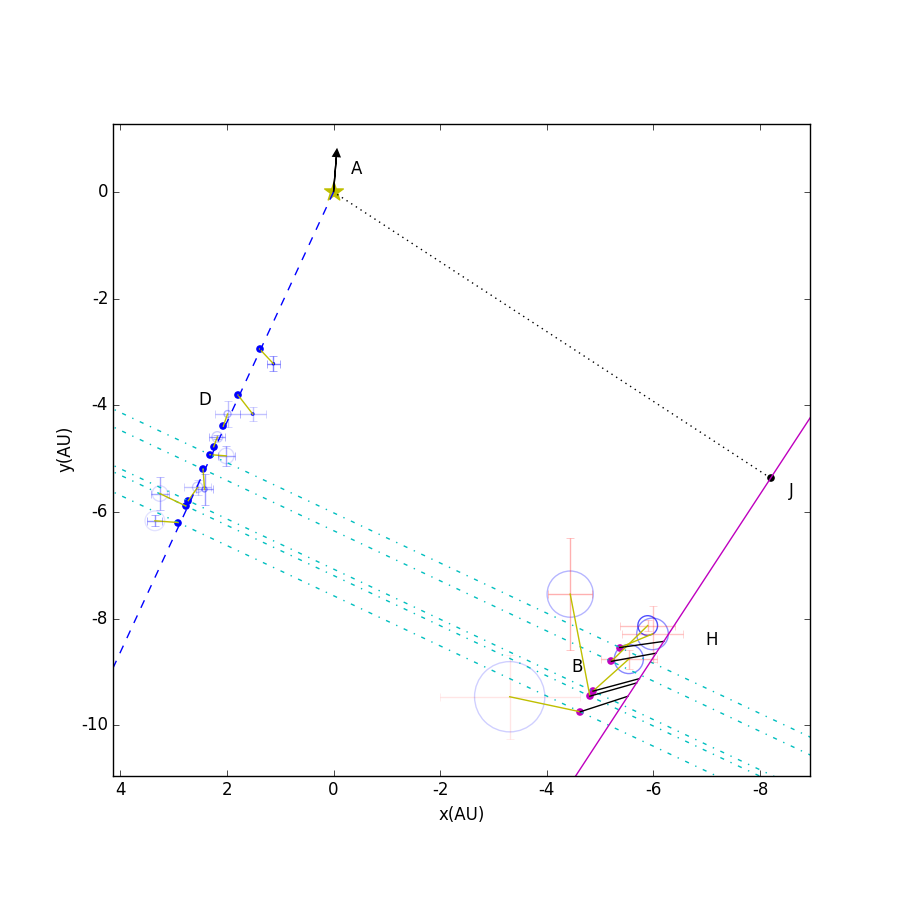
\includegraphics[width=1.0\textwidth, angle=0]{Double_lens_xy.png}
\caption{Observation data and calculated positions of $1$ ms and $0.4$ ms data of double lens model. In both apexes groups, the position of the screen locate at $392.8$ pc and $425.0$ pc. Blue points on the left side are the points that fitted from the $f_D$ and $\tau$ of from the $0.4$ ms apexes observation. Blue line is the fitted line of $0.4$ ms apexes positions, with a angle $\alpha$ $25.2$ degree west of north. The points lie on the left side with errorbars, are the observation points together with their sample errors; while the circles are plotted with population errors. Short solid lines between them are the matched positions of the observation positions and the calculated positions. The points on the right side are the points that fitted from the $f_D$ and $\tau$ of the $1$ ms apexes. Solid line is the fitted line of these positions. Those points with errorbars nearby are the observation points together with their sample errors, while the transparent circles are plotted with population errors. The dotted line on the top right side is vertical to the solid line. Short solid lines connect the observation points and the fitted positions. Middle lines connect the $0.4$ ms and $1$ ms fitted positions with the same $\theta_{\parallel}$. The proper motion of the pulsar is $192.6$ km/s, with an angle $\gamma$ $4.59$ degree west of north, is marked with an arrow from a star at the top of the figure.}
\label{Doublelens}
\end{figure*}


\begin{figure}
\centering
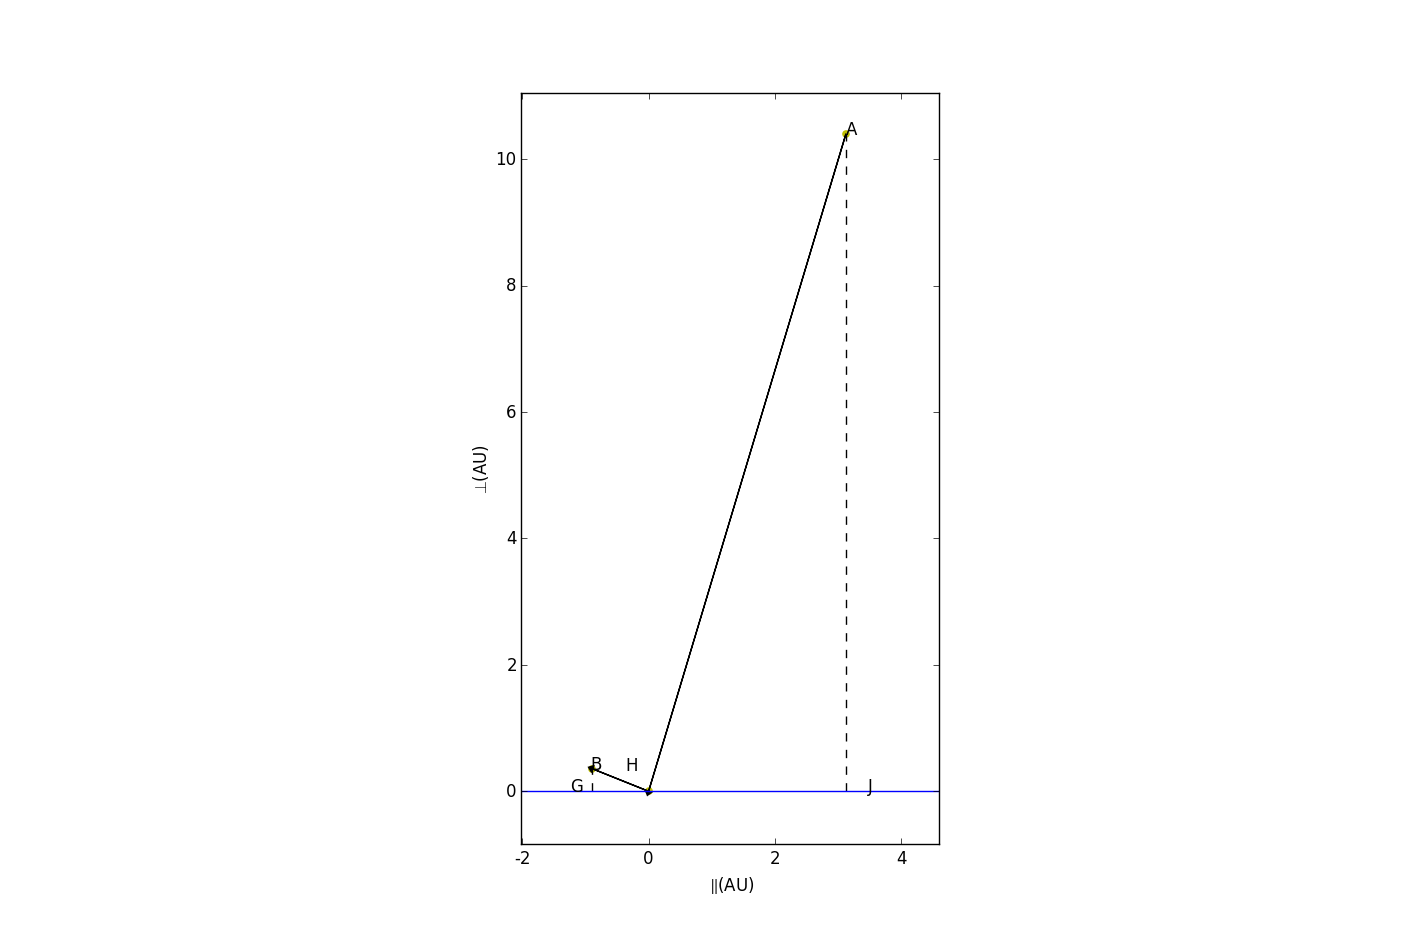
\includegraphics[width=1.0\linewidth,scale=1.0]{First_reflection.png}
\caption{Refraction on the far lens. The x axis marks the distance in the direction that is parallel to the first lens, and the y axis marks the distance in the direction that is transverse to the first lens. A is the position of the pulsar. H is the first screen image. B is the secondary screen iamge. J is the pedal of A to the first screen, and G is the pedal of B to the first screen. According to refraction Law, $v_{\rm JH}$ and $v_{\rm HG}$ should be equal. In this case, $\theta_{\parallel}$ of the second lens equal $-17.44$ mas.}
\label{first_reflect}
\end{figure}

\begin{figure}
\centering
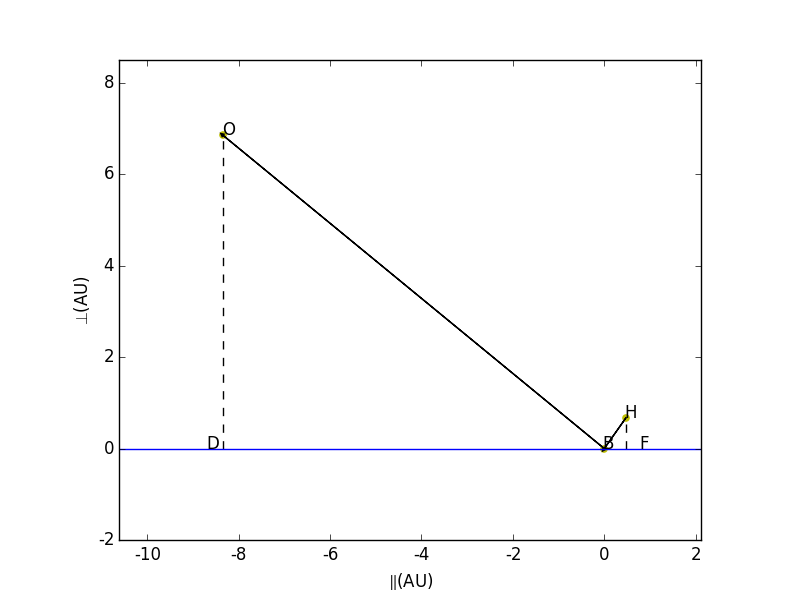
\includegraphics[width=1.0\linewidth]{Second_reflection.png}
\caption{Refraction on the near lens. x axis marks the distance in the direction that is parallel to the second lens, and the y axis marks the distance in the direction that is transverse to the second lens. H is the first screen image. B is the second screen image. O is the position of the observer. F is the pedal of H to the second screen, and D is the pedal of O to the second screen. According to the refraction law, $v_{\rm FB}$ and $v_{\rm BD}$ should be equal. In this case, $\theta_{\parallel}$ of the second lens equal $-17.44$ mas. }
\label{second_reflect}
\end{figure}

\begin{figure}
\centering
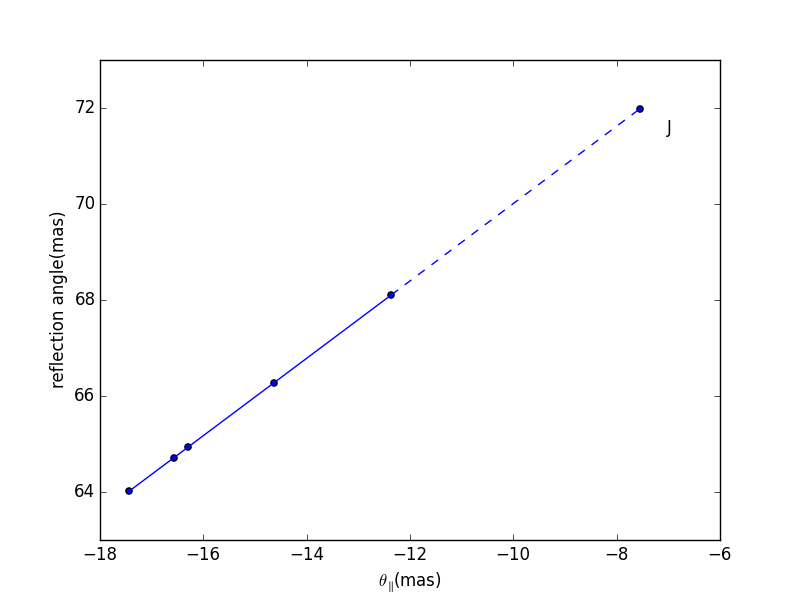
\includegraphics[width=1.0\linewidth,angle=0]{Reflection_angle.png}
\caption{Injection velocity minus refracted velocity over the speed of light. J specifically marked in the paper.}
\label{vtrans}
\end{figure}



\section{Possible Improvements}

We discuss several strategies which can improve on the solution
accuracy.  The single biggest improvement would be to monitor over a
week, when the pulsar crosses each individual lens, including both
lensing systems.

Angular resolution can be improved using longer baselines, for example
adding a GMRT-GBT baseline doubles the resolution.  Observing at
multiple frequencies over a longer period allows for a more precise
measurement: when the pulsar is between two lenses, the refraction
angle $\beta$ is small, and one expects to see the lensing at higher
frequency, where the resolution is higher, and distances between
lenses positions can be measured to much higher accuracy.

Holographic techniques \citep{2008MNRAS.388.1214W,2014MNRAS.440L..36P}
may be able to measure delays, fringe rates, and VLBI positions
sbstantially more accurately.  Combining these techniques, the
interstellar lensing could conceivably achieve distance measurements
an order of magnitude better than the current published effective
distance errors.  This could bring most pulsar timing array targets
into the coherent timing regime, enabling arc minute localization of
gravitational wave sources, lifting any potential source confusion.

Ultimately, the precision of the lensing results would be limited by
the fidelity of the lensing model.  In the inclined sheet model, the
images move along fold caustics.  The straightness of these caustics
depends on the inclination angle, which in turn depends on the
amplitude of the surface waves.  

\section{Conclusions}

We have applied the Pen and Levin \citet{2014MNRAS.442.3338P} inclined
sheet model to archival apex data of PSR B0834+06.  The data is well
fit by two linear lensing screens, with nearly plane-parallel
geometry.  This appears a natural consequence of very smooth
reconnection sheets, and are an unlikely outcome of ISM turbulence.
These results, if extrapolated to multi-epoch observations of binary
systems, this might result in accurate distance determinations.


\section{Acknowledgements}

We thank NSERC for support.


\newcommand{\araa}{ARA\&A}   % Annual Review of Astronomy and Astrophys.
\newcommand{\afz}{Afz}       % Astrofizica
\newcommand{\aj}{AJ}         % Astronomical Journal
\newcommand{\azh}{AZh}       % Astronomicekij Zhurnal
\newcommand{\aaa}{A\&A}      % Astronomy and Astrophysics
\newcommand{\aas}{A\&AS}     % Astronomy and Astrophys. Supplement Series
\newcommand{\aar}{A\&AR}     % Astronomy and Astrophysics Review
\newcommand{\apj}{ApJ}       % Astrophysical Journal
\newcommand{\apjs}{ApJS}     % Astrophysical Journal Supplement Series
\newcommand{\apjl}{ApJ}      % Astrophysical Journal Letters
\newcommand{\apss}{Ap\&SS}   % Astrophysics and Space Science
\newcommand{\baas}{BAAS}     % Bulletin of the American Astron. Society
\newcommand{\jaa}{JA\&A}     % Journal of Astronomy and Astrophysics
\newcommand{\mnras}{MNRAS}   % Monthly Notices of the Roy. Astron. Society
\newcommand{\nat}{Nat}       % Nature
\newcommand{\pasj}{PASJ}     % Publ. of the Astron. Society of Japan
\newcommand{\pasp}{PASP}     % Publ. of the Astron. Society of the Pacific
\newcommand{\paspc}{PASPC}   % Publ. Astron. Soc. Pacific Conf. Proc.
\newcommand{\qjras}{QJRAS}   % Quart. Journal of the Royal Astron. Society
\newcommand{\sci}{Sci}       % Science
\newcommand{\solphys}{Solar Physics}       % 
\newcommand{\sova}{SvA}      % Soviet Astronomy
\newcommand{\aap}{A\&A}
\newcommand\jcap{{J. Cosmology Astropart. Phys.}}%
\newcommand{\prd}{Phys. Rev. D}


\bibliography{distance}
\bibliographystyle{mn2e}


\label{lastpage}

\end{document}
